\documentclass{standalone}
\usepackage{tikz}
\usetikzlibrary{positioning, shapes.geometric, arrows.meta}

\begin{document}
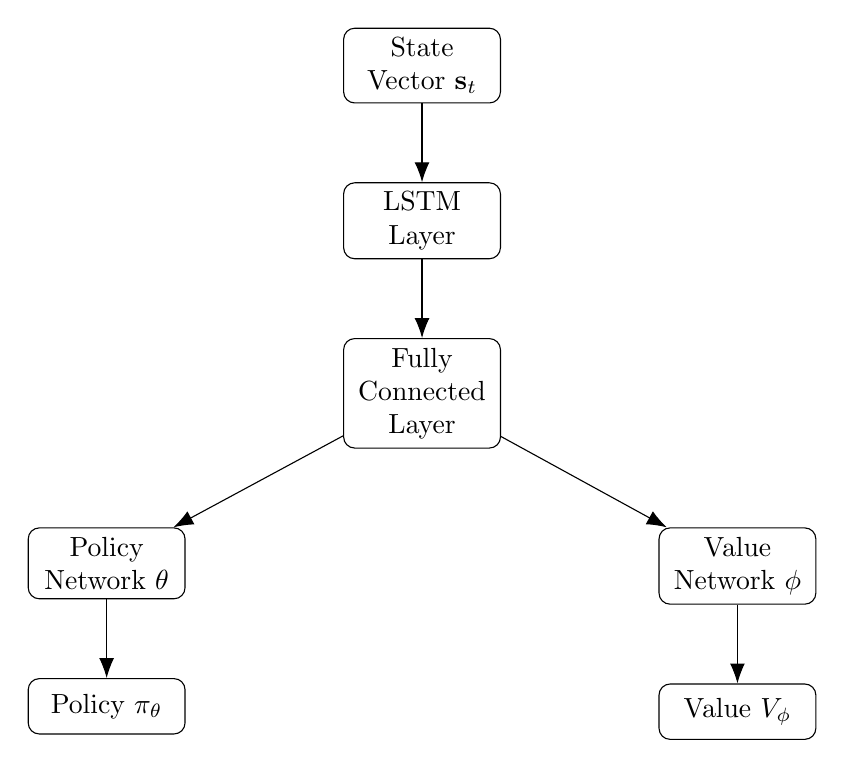
\begin{tikzpicture}[
    node distance=1cm and 3cm,  % Reduced vertical spacing, keep horizontal spacing
    every node/.style={align=center},
    block/.style={rectangle, draw, text width=5em, text centered, rounded corners, minimum height=2em},
    line/.style={draw, -{Latex[scale=1.5]}}
]

% Nodes
\node[block] (input) {State Vector $\mathbf{s}_t$};
\node[block, below=of input, yshift=0cm] (lstm_layer) {LSTM Layer};
\node[block, below=of lstm_layer, yshift=0cm] (fc_layer) {Fully Connected Layer};
\node[block, below left=of fc_layer, xshift=1cm, yshift=0cm] (policy_hidden) {Policy Network $\theta$};
\node[block, below right=of fc_layer, xshift=-1cm, yshift=0cm] (value_hidden) {Value Network $\phi$};
\node[block, below=of policy_hidden, yshift=0cm] (policy_output) {Policy $\pi_\theta$};
\node[block, below=of value_hidden, yshift=0cm] (value_output) {Value $V_\phi$};

% Arrows
\path[line] (input) -- (lstm_layer) node[midway, left] {};
\path[line] (lstm_layer) -- (fc_layer) node[midway, left] {};
\path[line] (fc_layer) -- (policy_hidden) node[midway, left] {};
\path[line] (fc_layer) -- (value_hidden) node[midway, right] {};
\path[line] (policy_hidden) -- (policy_output) node[midway, left] {};
\path[line] (value_hidden) -- (value_output) node[midway, right] {};

\end{tikzpicture}
\end{document}
